% !TeX root = ../main.tex
% Add the above to each chapter to make compiling the PDF easier in some editors.

\chapter{Background and Related Work}\label{chapter:background}

This chapter describes the concepts and background information that this thesis uses and relies on. It gives a brief introduction about Internet of things and other concepts such as pervasive and fog computing in addition to  explaining Delay-Tolerant and Information-Centric Networking as they play an important role in this thesis. Further, we explain the software platforms and hardware used to implement the proposed framework.

\section{Internet of Things}

In general terms, IoT refers to a highly dynamic and scalable distributed network of connected devices equipped with context-aware gadgets that enables them to see, hear and think \cite{DAC:DAC2417}. Then, transform these senses to a stream of information allowing them to digest the data and act intelligently through actuators if needed. They are also allowed to communicate and share knowledge, which make them smart, powerful and capable of acting independently. Smart devices in an IoT network are heterogeneous in terms of computation capabilities, also each device is energy optimized and able to communicate. Additionally, to qualify for being smart, devices must have a unique global identifier, name, address and can sense the environment. However, the IoT network may also contain devices that are not "smart" which act upon receiving orders triggered through certain circumstances in the network, for example, a lamp post that is set on and off according to network signals. \\

\noindent Since smart devices have unique identifiers and are context-aware, they can be tracked and localized, which is very helpful when performing geospatial computations \cite{Miorandi20121497}. The huge demand on IoT has triggered the development of small-scale, high-performance, low-cost computers, in addition, sensors and actuators are getting cheaper, smaller and more powerful which in turn increased the interest even more.\\
 

\noindent The IoT concept can be viewed from different perspectives, it is very elastic and provides a large scale of opportunities in many areas. Currently the number of connected smart devices are estimated in billions, they aim to automate everything around us and are mainly targeted to increase life quality. The broad range of IoT applications include:
\begin{itemize}
\item Smart homes which tend to use sensors and actuators to monitor and optimize home resource consumption and control home devices in a way that increases humans satisfaction. Further, expenses generated from resource usage such as gas, power, water and telecommunications can be sent directly to related authorities without any human intervention \cite{Chan:2008:RSH:1377032.1377113}.  
\item Smart factories also known as "Industry 4.0" the fourth industrial revolution which are optimized machines that communicate together in order to improve the manufacturing process and gather data to analyze factories logistics, pipeline and product availability. It also creates intelligent products that can be located and identified at all times in the process \cite{Gilchrist:2016:III:2994178}.

\item Smart cities is one of the most adopted applications in the IoT field, it comprises smart parking, traffic congestion monitoring and control, real time noise analysis, waste management and others.  All this applications need enhanced communication and data infrastructure. It aims to increasing quality of living for individuals \cite{6740844}. 

\item There are also applications in  health care, environmental monitoring, security and surveillance.
\end{itemize}

\noindent IoT is very diverse, one way of applying it is to gather data from the smart devices, then process data in the cloud via \textit{Cloud Computing}. Afterwards, results could be sent back to smart devices in order to act somehow. Nevertheless, there are approaches for pushing computations to the smart devices "Edges"  such as 
\textit{Edge Computing}, \textit{Pervasive Computing} and \textit{Fog Computing} emerged.



\subsection{Pervasive Computing} 
 Pervasive computing, also known as \textit{Ubiquitous Computing}, is a concept in which software devices and agents are expected to support and act upon human needs anytime and anywhere without their interference \cite{Chen:2003:OCP:991804.991806}. It is usually integrated with intelligent agents and smart devices which keep learning from human actions and the decisions taken previously to be even more helpful every time. Also, pervasive software agents are context-aware in most of the cases, in which they know what changes are happening around them at a specific point in time and hold a history of what has happened in the environment. They also communicate seamlessly in order to share knowledge and help each other take better decisions. Moreover, pervasive devices can be relocated from one place to another, thus changing the network and possibly the environment. Therefore, devices can not be addressed with their respective networked addresses because they might eventually change. \\

\noindent In 1991 Mark Wieser said in the paper describing his vision of ubiquitous computing  \say{The most profound technologies are those that disappear. They weave themselves into the fabric of everyday life until they are indistinguishable from it} \cite{weiser1991ubicomp}. Since then, computing has evolved from using only desktop personal computers to the current phase of wireless sensor networks, small computational devices and distributed systems. Imagine the large scale of applications that could incorporate the computational power, artificial intelligence, machine learning and context-awareness to serve human beings without them even noticing that it exists. In the same paper Wieser also concluded \say{Most important, ubiquitous computers will help overcome the problem of information overload. There is more information available at our fingertips during a walk in the woods than in any computer system, yet people find a walk among trees relaxing and computers frustrating. Machines that fit the human environment, instead of forcing humans to enter theirs, will make using a computer as refreshing as taking a walk in the woods.}\\



\noindent Figure \ref{fig:pervaisive-computing} shows the architecture of a pervasive environment, in which devices are connected together through a pervasive network which should be lenient to relocating. In addition, each pervasive device has several applications that depend on environment and  context. The pervasive middleware is an abstraction of the core software to the end-user applications.

\begin{figure}[H]
	\centering
	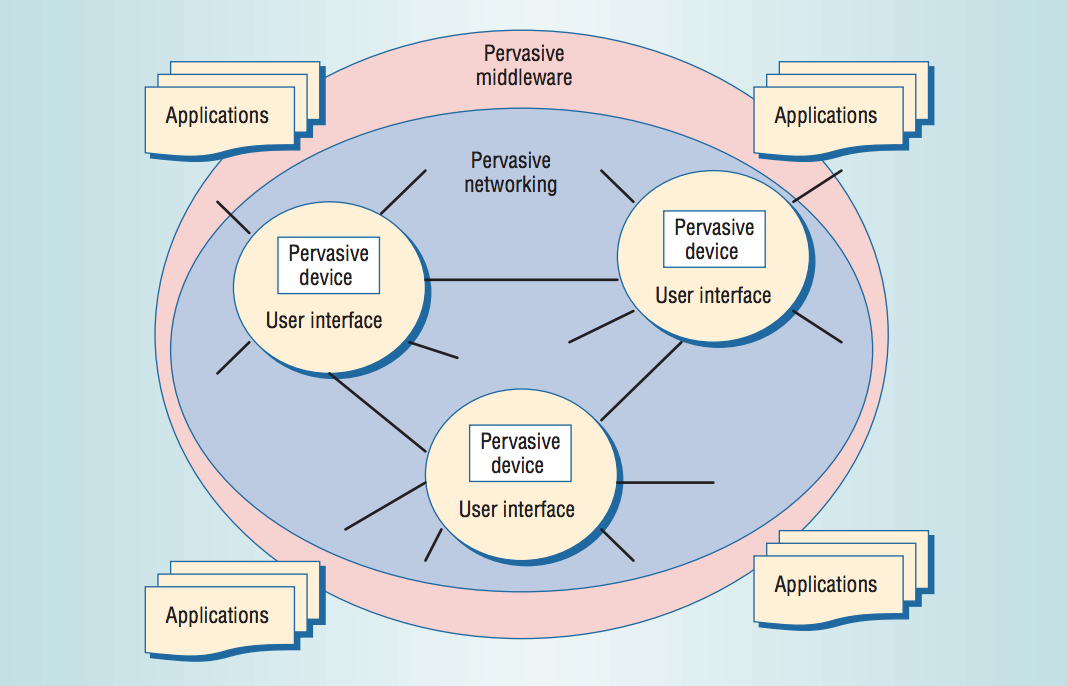
\includegraphics[scale=0.7]{images/pervasive-computing.png}
	\caption{Pervasive Computing environment architecture. \textit{Adopted from \cite{Saha:2003:PCP:642243.642248}}.}
 	\label{fig:pervaisive-computing}
\end{figure}

\noindent The road to pervasiveness is not paved with gold, there are many challenges that faces the design and implementation of pervasive applications. Some of these challenges are \cite{Schiele2010}:
\begin{enumerate}
\item Devices have become more heterogeneous and the middleware must be able to execute on each of them, therefore, the use of self-contained software environments is advised.
% For example, using docker as an execution environment for all the heterogeneous devices.
\item Communication reliability is often questioned, in addition,  environments are highly dynamic thus devices are only known at run time.   Therefore, service discovery is a must, either peer-based in which all nodes  take part in the discovery or mediator-bases in which some special devices are promoted to perform service discovery.
\item Sensor availability on smart devices, readings uncertainty of sensors and continuous update of user requirements.
\item Communication and cooperation between devices requires interoperability. There are three different ways that allows them to cooperate:

\begin{itemize}
\item Fixed standardized protocol, in which we set some technologies, protocols and data formats in order to be used across the system.
\item Dynamically negotiated, in which devices are allowed to negotiate on which protocols and data formats to use  at run time.
\item Using interaction bridges that map between different approaches and protocols.
\end{itemize}

\end{enumerate} 



\subsection{Fog Computing}

The fog is an extension to cloud computing at the edge of the network. It provides computation, storage, networking and application services to end-users. Fog and cloud are independent, in fact, cloud can be used to manage the fog. They are also mutually beneficial, some use cases are better deployed in the fog and vice versa. Research yet to determine which applications should go where. The fog is characterized by having lower latency than the cloud, thus are more useful in time critical applications. Also, fog devices have location awareness with a better geographical distribution than the centralized cloud approach. It can distribute the computations and storage between the cloud, itself and idling devices on the network edge \cite{7498684}. However, it remains a challenge to deal with all the heterogeneous devices in the fog. Connecting various components with different nature ensuring quality of service is not easy. Moreover, a unified programming model should be used in all fog devices in order to help programmers make use of the fog model. Other issues are also being researched such as security and privacy of the fog network \cite{Yi:2015:SFC:2757384.2757397}. 



\section{ Messaging Protocols}
With the rise of IoT and the need for interoperability and seamless communication between smart devices, researchers and professionals have been working on developing messaging protocols that aim to aid in Machine-To-Machine (M2M) communication without any human interaction. The M2M messaging approaches can be divided into two main categories, broker and broker-less.\\

\noindent The broker architecture means that there is a server in the middle of all communication acting as a "broker". Every machine in this architecture is connected to this broker and every message whether a publish or subscribe goes through it. The advantages of this model is that, machines do not need service discovery for peers, the only thing they need to know is the broker's address. Further, if one machine published a message to the broker and died, it can still reach a receiver ("even if not yet online") through the broker, it can also provide a delivery guarantee. However it has some disadvantages,  there is an extensive network communication that goes through the broker, thus it becomes a bottleneck, though there is a possibility to have multiple brokers in a single network.  Also, in a dynamic environment the broker or brokers addresses might not be known beforehand therefore it becomes very hard to set up broker architecture in this environment. MQTT \cite{mqtt} and AMQP \cite{amqp} are examples of this approach protocols.\\

\noindent The broker-less architecture means that machines communicate directly to each other or through multiple hops, thus it relies heavily on peer discovery. It tackles the bottleneck of broker network communication, since messages only have to go from publishing peers to interested ones.  Furthermore, since machines are not always available, therefore the architecture needs to deal with unavailable machines which may not have started. In addition, it has to handle message delivery to machines with no end-to-end path or direct connectivity. ZeroMQ \cite{zeromq} is one implementation of broker-less architectures. \\


\noindent There is a third category which is endpoint centric such as RESTful services, web sockets and protocols like Constrained Application Protocol CoAP \cite{coAP} that uses the REST architectural style and is built over UDP. It also supports service discovery, multicast and asynchronous messaging exchange. 

\section{Networking}

The following is a brief introduction of the main networking grounds that are used in this thesis. Since, the  proposed software framework focuses on exchanging data and computation between nodes even without an end-to-end path, its imminent that we shed light on Information-Centric Networking which proposes replacing current host-centric  Internet architecture  with a content-centric one. Additionally,  having no end-to-end paths between some  of our nodes, guides us to leverage the concept of Delay-Tolerant Networking that can store messages and carry it forward even without a connection through mobile devices.
\subsection{Information Centric Networking}

Information-Centric Networking (ICN) is an architecture that focuses on \textit{WHAT} information is being exchanged rather than \textit{WHO} are exchanging it. ICN was mainly described by Dirk Trossen et al. as a networking architecture that aim to replace the current Internet inter-networking layer using publish-subscribe model as an underlying service \cite{Trossen:2010:AII:1764873.1764878}. Trossen introduced four main challenges that faces the architecture which are namely information-centrism of applications, supporting and exposing tussles, increasing accountability, and addressing attention scarcity.
\begin{figure}[H]
	\centering
	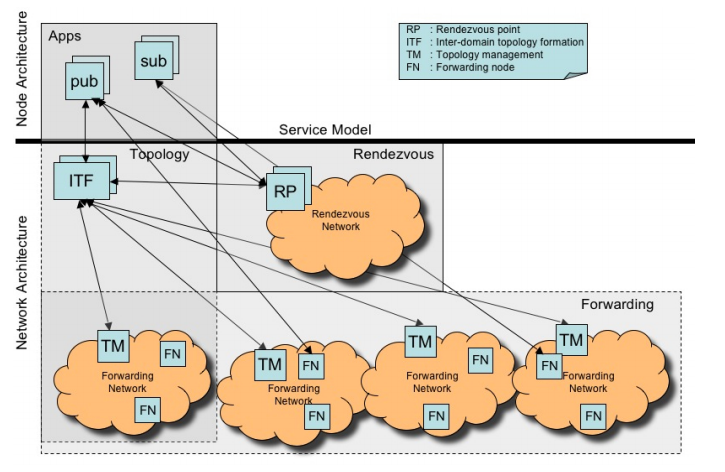
\includegraphics[scale=0.4]{images/trossen.png}
	\caption{ICN architecture by Dirk Trossen et al. \textit{Adapted from } \cite{Trossen:2010:AII:1764873.1764878}.}
	\label{fig:trossen}
\end{figure}

\noindent The architecture  design has three main functions:
\begin{itemize}
\item \textit{Rendezvous}: which are used to match  publishers and subscribers of information, each of them is identified by a globally unique identifier called Rendezvous Identifier (RI). The information items required to perform this matching exists in the Rendezvous Points (RP).
\item \textit{Forwarding Topology}: which is created once there is a match between publications and subscriptions in cooperation with the inter-domain topology formation (ITF). It depends on the publishers and subscribers location on the level of Autonomous Systems (AS).
\item \textit{Topology manager}: which resides in each AS and is used as a transfer link between ASes. Also, it is used to guide Forwarding Nodes (FN) to create a route between local publishers and subscribers.
\end{itemize}


 		 
\noindent ICN  is content-centric in contrast to current network approaches which are  host-centric, wherein communication takes place between hosts such as servers, personal computers, etc. ICN was brought to light as a result of the increasing demand on content sharing in highly scalable, distributed and efficient fashion. It compromises network caching, replication across entities and resilience to failure. The content types includes web-pages, videos, images, documents, streaming and others which are titled Named Data Objects (NDOs). The NDO is only concerned by its name and data. As long as the name identity is preserved, it does not matter where the NDO is going to be persisted, what is the storage method or which type of transport procedure is used. Therefore, copies of NDO are equivalent and can be supplied from any location or replica across an ICN network. However, since the name represents its identity, ICN requires unique naming for individual NDOs.\\

\noindent ICN also provides an Application Programming interface (API) that is responsible for sending and receiving NDOs. The two main roles in this API are the producer who produces content to a specific name and the consumer who asks if an NDO is available by its name. There is also the publish-subscribe approach in which a consumer registers for a subscription to a certain name and gets notified whenever new content is available. This caters for  decoupling between producers and consumers.\\

\noindent To ensure that an NDO goes from one entity to another, a consumer request must go through two different routing phases. The first is to find a node that holds a copy of the  NDO
and deliver the request to that node. The second is to find a routing path back from the receiving node to requester carrying the required NDO. This can be achieved in two different ways: i) \textit{name-resolution} in which a resolution service is queried in order to find a way to locate a source node, ii) \textit{name-based routing} in which the request is forwarded to	 another entity on the network based on routing algorithms, policies and cached information. \\

\noindent ICN caches are available on all nodes, requests to an NDO can be served from any node having a copy in the cache. An NDO can be cached on-path from sender to receiver or off-path through routing protocols or by registering it into a name-resolution service \cite{6231276}.


\subsubsection{Content Centric Networking}
Content-centric networking (CCN) was first introduced by Van Jacobson et al., in order to tackle current network architecture issues such as availability, security and location independence. The main communication model relies on two main CCN packets namely \verb|interest| and \verb|data| packets. It works as follows, a consumer broadcasts its interest of information to all connected nodes. If a node posses the desired data and received an interest packet, it responds with a data packet \cite{Jacobson:2009:NNC:1658939.1658941}.\\

\noindent CCN is  based on the ICN concept, namespace in CCN  is hierarchal, for instance, \verb|/tum.de/connected-mobility/iot| matches the Figure \ref{fig:ccn-namespace}. Names do not have to be meaningful or readable, they can include hashes, timestamps, ids, etc. A request matches an NDO if its name is a prefix of any named object, for example,  a request with the name  \verb|/tum.de/connected-mobility/iot| matches an NDO with the name  \verb|/tum.de/connected-mobility/iot/pervasive-computing|. CCN natively support on-path caching with name-based routing, however, off-path can also be supported \cite{6563278}.
\begin{figure}[H]
	\centering
	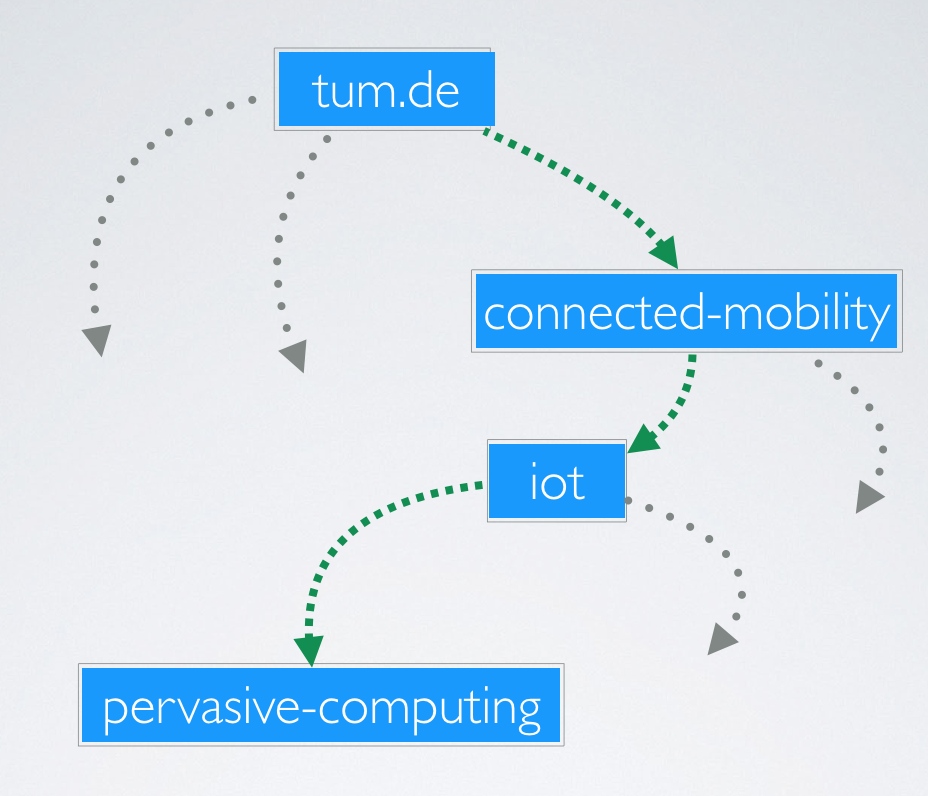
\includegraphics[scale=0.3]{images/namespace.png}
	\caption{Hierarchal namespace example for CCN.}
	\label{fig:ccn-namespace}
\end{figure}

Each node in the network contains a \textit{Content Router} which includes three data structures \cite{6563278}\cite{6231276}. 
\begin{itemize}
\item \textit{Pending Interest Table (PIT)}: which stores the subscriptions and interests of NDOs. The subscription does not have to originate  from the node itself, rather can be a forwarded from another node. Once an interest reaches a content source and the data is retrieved, the PIT entries serves as a trail to the original subscriber and is removed afterwards.

\item \textit{Forwarding Information base (FIB)}:  stores a mapping that indicates which node should the request be forwarded to. The FIB uses longest common prefix in order to determine the next hop. Multiple entries are allowed and can be queried in parallel.

\item \textit{Content Store (CS)}: which is basically the cache that stores the NDOs and uses \textit{least recently used} (LRU) eviction strategy. Caches with high hierarchy posses a larger storage to be able to store popular NDOs which might get evicted due to  lower storage down in the hierarchy.
\end{itemize}  

\begin{figure}[H]
	\centering
	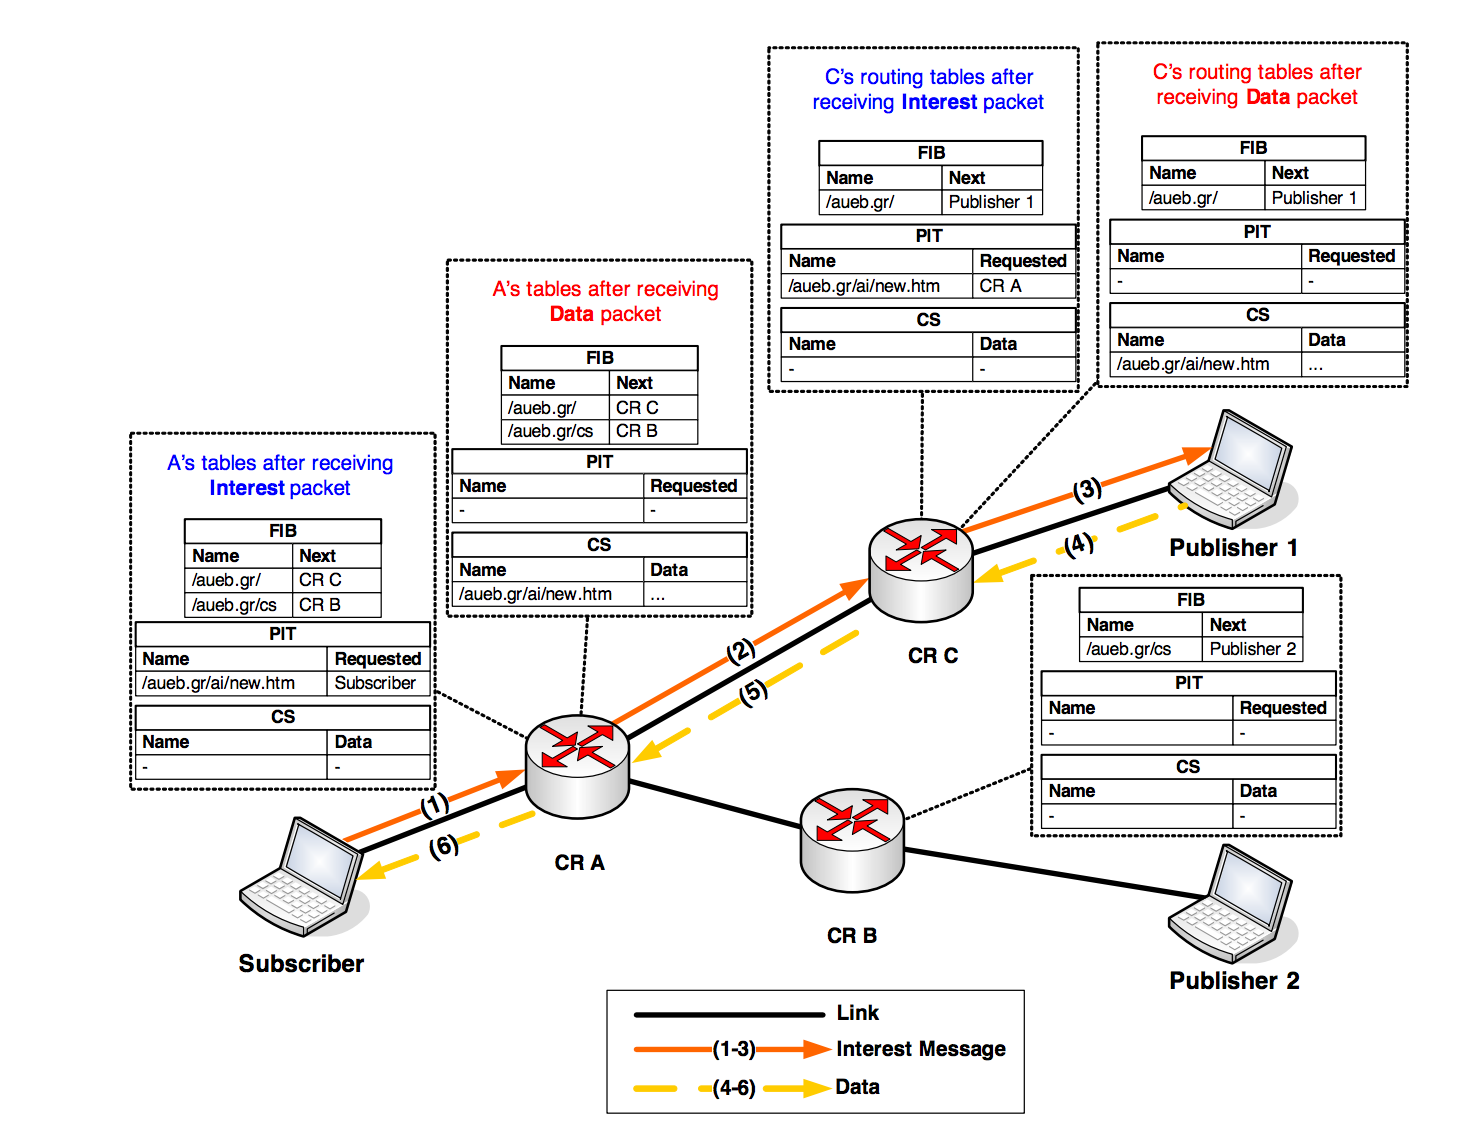
\includegraphics[scale=0.4]{images/ccn2.png}
	\caption{Content centric networking architecture and flow. \textit{Adopted from \cite{6563278}}.}
	\label{fig:ccn}
\end{figure}

\noindent Figure \ref{fig:ccn} describes the flow and state of PIT, FIB and CS of network nodes when receiving the interest message and after acquiring the data. Notice that, all the PIT entries have been erased after acquiring the data and CSs have been updated.


\subsubsection{Networking of Information }
Network of Information (NetInf) is an architecture based on the ICN concept. Unlike CCN, routing in NetInf is a hybrid of name-based  and the name-resolution scheme, also, NDO names are not human readable. Namespace is not hierarchal rather flat, however, there is one common naming format for all NDOs across all nodes. Moreover, it supports on-path and off-path caching \cite{Dannewitz:2013:NII:2459510.2459643}. In Figure \ref{fig:netinf}, there are two requests namely \textbf{A} and \textbf{B}.  NetInf used name-resolution service (NRS) to get the source location of \textbf{B}. Alternatively, it used name-based routing (NBR) in combination with NRS to find the request source of \textbf{A}.

\begin{figure}[H]
	\centering
	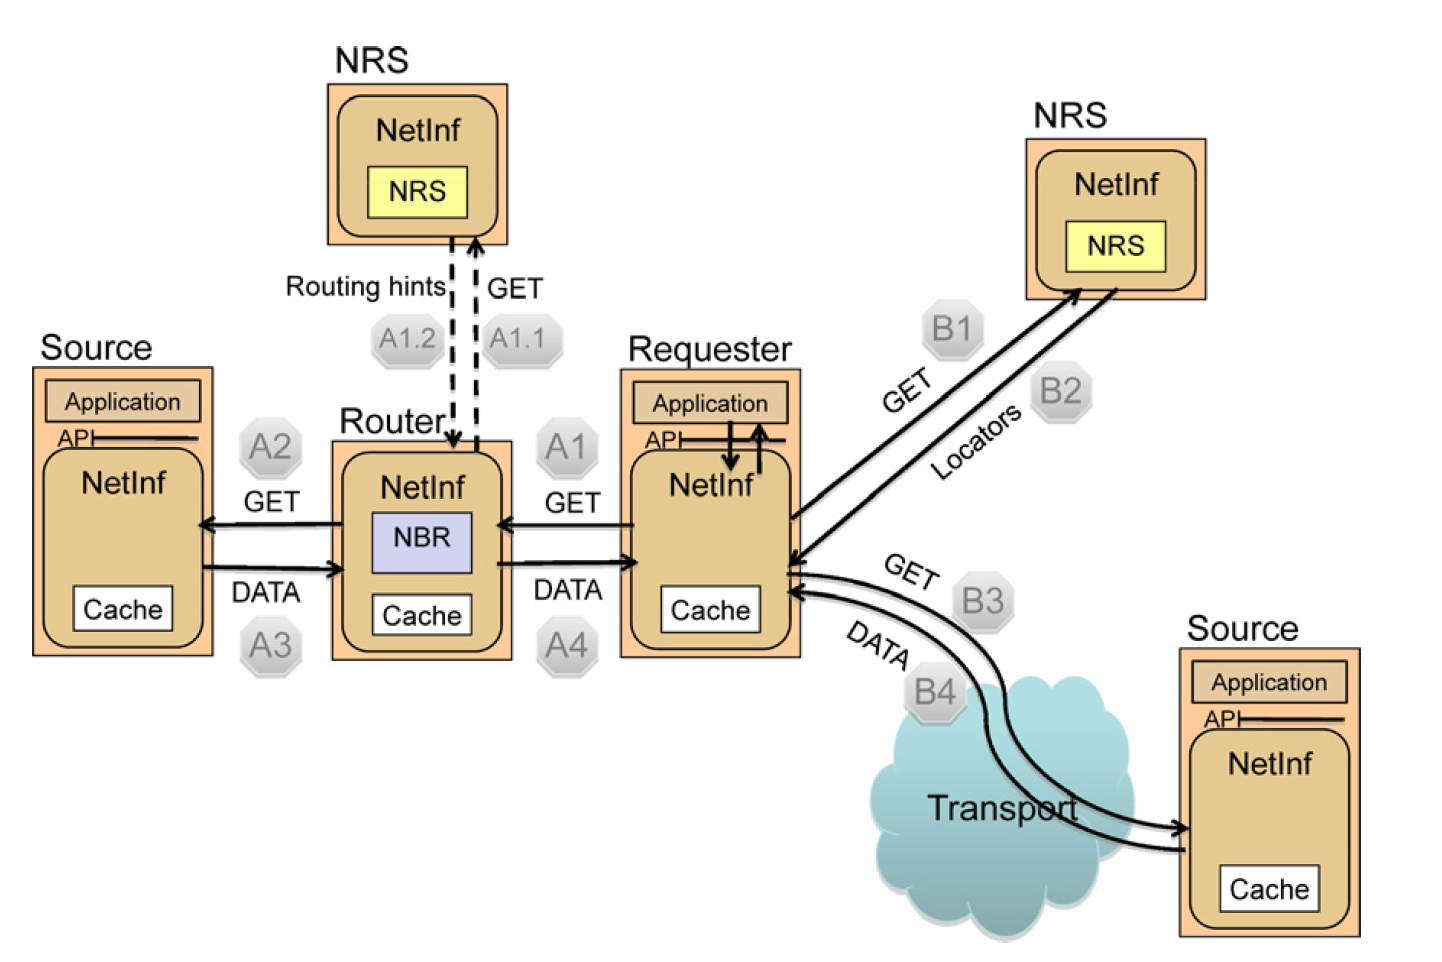
\includegraphics[scale=0.4]{images/netinf.png}
	\caption{NetInf routing flow example. \textit{Adopted from \cite{Dannewitz:2013:NII:2459510.2459643}}.}
	\label{fig:netinf}
\end{figure}



\subsection{Delay Tolerant Networking}

Delay-Tolerant Networking (DTN) is an overlay architecture proposed to overcome unreliable connections between nodes through asynchronous message forwarding. In some challenged networks, there might not exist an end-to-end path between nodes either wired or not. Further, valid connections might exhibit extensive delays which might not be acceptable and thus cause the message transfer to drop. By an overlay architecture it is meant that DTN functions resides above the existing protocol stacks thus achieving interoperability and providing the store-carry-forward functionality \cite{Fall:2003:DNA:863955.863960}.\\

\noindent The DTN Research Group (DTNRG) has proposed an architecture which was published as Request For Comments (RFC) to the Internet Engineering Task Force (IETF). The architecture defines an end-to-end message-oriented overlay called "bundle layer" which is located  between  application layer and  transport layer. The bundle layer encompasses a persistent storage, basic security model and store-and-forward routing to overcome disconnected and disrupted communications. Devices implementing the bundle layer are called DTN nodes and are bound to the Bundle Protocol \cite{scott2007bundle}. Data units exchanged between these layers are named "bundles",  which are messages containing a header, user application's data and control information such as how to handle, store and dispose of user data. Bundles can also be divided into fragments  to increase delivery performance which are assembled again at the destination. Fragments are also bundles themselves, two or more of them can be re-assembled anywhere in the network to create a bundle. Bundles contain identifiers which distinguish the original sender and final destination. DTN nodes can store and persist bundles over longer time periods until a connection is regained.  Persistence allows DTN nodes to recover from system restarts \cite{fall2007delay}.\\


\noindent There are different implementations of the DTN architecture. DTN2 is a reference implementation by the DTNRG to demonstrate the basic functionalities thus the performance is not optimized. There are also ION and DTNLite, however, they do not allow the use of common programming languages. IBR-DTN is yet another implementation designed for embedded systems, it also has discovery via broadcasting \cite{Doering:2008:IEI:1409985.1410008}. Also, SCAMPI application platform which will be explained in details.




\section{Used Platforms}
Turning now to explain the platforms that we used in order to implement our framework. The section includes a hardware component which is the Raspberry Pi and all the other components are software oriented. This includes SCAMPI publish-subscribe platform for message passing in delay tolerant networks, node-RED project for wiring IoT applications and time-series databases.

\subsection{SCAMPI}
SCAMPI is a delay tolerant platform based on the DTNRG architecture that hides networking from the application user \cite{Karkkainen:2012:SAP:2348616.2348636}. It enables communication between peers even without and end-to-end path. The store-carry-forward router implemented by SCAMPI empower peer discovery via broadcast, mutlicast, TCP unicast  and subnet scanning for known ports. In addition, it offers caching and multi-hop message transfer. Unlike DTN2 and IBR-DTN which exchanges payloads as blobs of data, SCAMPI supports structured data messages as map where arbitrary string keys map to binary buffers, strings, numbers or file pointers. SCAMPI also provides the entity SCAMPIMessage that maps to the Bundle Protocol in the DTN architecture. Moreover, the SCAMPIMessage entity can carry meta-data that describes the content. \\

\noindent SCAMPI is also based on the information-centric architecture in which it provides an API (over TCP) that allows broker-less publish-subscribe service of messages using NDO names that can be human readable or hashes. Additionally, it supports automatic framing of structured messages, searching for content based on message meta-data and peer discovery of nearby nodes. The TCP API works as an interface that can be implemented by any application written in any programming language. SCAMPI is Java based, therefore, the Java Virtual Machine (JVM) is the only requirement to have SCAMPI up and running. Furthermore, there is an android application that runs  a persistent background process SCAMPI router, allowing android phones to route data through the native TCP API. Having SCAMPI running on the android phone allows it to carry messages from one endpoint to another without even having neither wired connection or a wireless one between the sender and receiver, simply the phone is used to carry the data from one network to another. \\

\noindent Extending DTN and ICN, we think that SCAMPI is the best platform to use for this thesis. The are several reasons for that, firstly being a DTN, SCAMPI provides reliability for delivering messages even when there is no end-to-end path or connection is disrupted. Secondly, using peer discovery allow us to add or remove pervasive agents at-will. Thirdly, as our approach is information-centric, it is handy that SCAMPI allows the publish-subscribe messaging scheme on top of the DTN architecture. 


\subsection{Raspberry Pi}
Raspberry Pi is a very small, low-cost and single-board computer that was originally developed to promote computer science education in schools by the Raspberry Pi Foundation. It has a rather low processing power and random access memory compared to todays computers and mobile devices. Nevertheless, its graphical processing units equals that of todays latest mobile devices, it can stream high definition videos and run 3D games. Raspberry Pi also has 40 General Purpose Input/Output (gpio) pins that act like switches in order to send signals to devices such as LED lamps, sensors and actuators which makes it suitable for the IoT applications. Further, there are lightweight operating systems deigned especially to cope with the edge devices and the Raspberry Pi  such as \textit{Ubuntu MATE},  \textit{Windows 10 IoT Core} and \textit{Raspbian} which is officially supported by the foundation.
\begin{figure}[H]
	\centering
	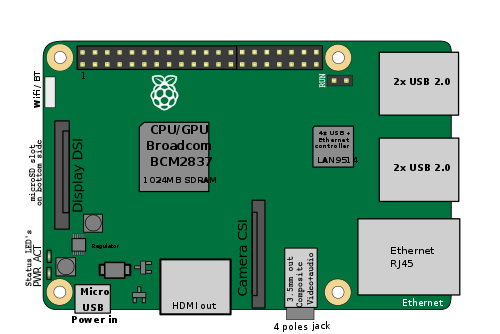
\includegraphics[scale=0.5]{images/rpi.png}
	\caption{Raspberry Pi  3 model B design. \textit{Adopted from \cite{RASPI}}.}
	\label{fig:rpi}
\end{figure}
\noindent In this thesis we use the Raspberry PI 3 model B as shown in Figure \ref{fig:rpi} with the following specifications:
\begin{itemize}
	\item 1.2 GHz processor designed by ARM and 1 GB of random access memory.
	\item Ethernet port, wireless LAN, Bluetooth 4.1 and Bluetooth low energy to enable wide range of connectivity.
	\item Micro-SD card slot for storage and hosting the operating system.
	\item Audio jack, HDMI port and 4 USB ports.
	\item Camera, display interface and 40 gpio pins.
\end{itemize}

\noindent There are other models of the Raspberry Pi such as  Pi 2 Model B,  Pi Zero, and  Pi 1 Model B+ and A+, they differ in size and specification. However, they all share the same concept of being low-cost and single-board computers \cite{RaspberryPi}.



\subsection{Node-RED}
Node-RED \cite{NODE-RED} is a powerful, open-source and flow-based programming project originally developed by IBM Emerging Technology Services and now a part of the JS foundation designed for IoT. Flow-based programming describes an application as a network of black-box nodes that exchange data together.  Node-RED is widely used as a visual tool for wiring IoT applications that can be deployed locally, on the cloud or on edge devices such as (Raspberry Pi, Android, Arduino). Nodes are the building blocks of node-RED, each has its own defined purpose and can be given a certain input which in turn can give an output. Further, these nodes can be re-used and  have different visuals which makes them easy to use and more handy for a wider range of users. The function of these nodes varies from digital, social  or even physical events that include sensors. The network of nodes is called a  \textit{flow}, flows can be  serialized into JSON objects and thus simplifying  importing, exporting and sharing process. Since node-RED is an open-source project which is very well adopted. Therefore, the community is allowed to create new flows and extend current ones for their own use cases and make them available to the public, they are also allowed to report potential problems and bugs to the contributers. This results in a very fast development, fixes, new features and releases.\\

\noindent Node-RED user interface is available through the browser via \verb|localhost:1880| where \verb|1880| is the default port, however, there is an API to import and export flows through node-RED engine without using the user interface. Figure \ref{fig:node-red} shows the browser window with node-RED UI. On the left side exists the nodes which represent the building blocks of the flow, they can be dragged and dropped inside the empty canvas. Afterwards, nodes can be wired together and deployed. In the figure, a simple flow including a time-stamp triggered every five seconds and debug node are wired together and deployed. On the right side of the figure, printed time-stamps can be seen in the debug pane as a result of wiring the debug element into the flow and connecting it to the configured time-stamp element. The Info tab on the right side, explains each node once it is selected, shows its documentation and how to use it.


\begin{figure}[H]
	\centering
	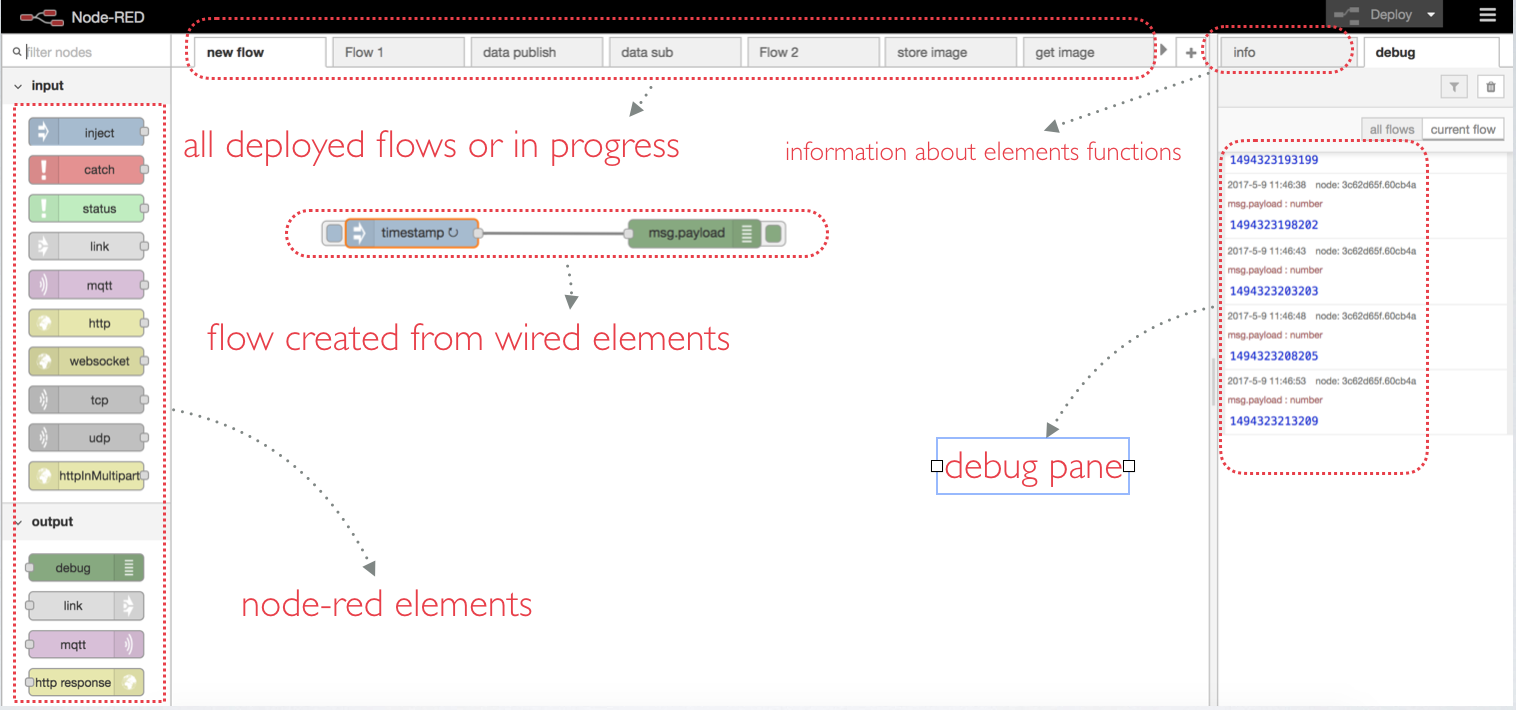
\includegraphics[scale=0.5]{images/node-red.png}
	\caption{Node-Red user interface to create and deploy flows for IoT applications.}
	\label{fig:node-red}
\end{figure}


\noindent Node-RED also allows global context, meaning, we can set custom variables that live across all nodes. This is really helpful when  an application should keep a certain shared state. The main programming language of node-RED is JavaScript, it is also possible to write a custom node which executes code or script of any language through the execute node and the result can be  wired inside the flow. Moreover, node-RED has a built-in node to control gpio pins of a Raspberry Pi, that can send low or high signals whenever desired to a certain pin. This is powerful because it hides the abstraction behind controlling the Raspberry Pi  pins.\\


\noindent Given its features and specifications, our proposed framework uses node-RED as an environment for deploying computations, in other words, each smart device in our architecture must have a node-RED instance. Hence, we could use  flows and wired nodes to express computations and serialize it via the export feature. Thereafter, we could send serialized computations along with their dependencies, meta-data  to other nodes running node-RED instances and deploy the computation on them. 

\subsection{Time-series Databases}

Time-series databases are optimized for storing  and fetching data which is collected in a timely based manner, in other words, data which is timestamped. They are intended to handle huge volume of data especially for monitoring, real-time analytics and continuous measurement of IoT sensor data. Manipulating time-series data like aggregating, creating subsets and re-sampling can be a tricky task \cite{Leighton2015}. Time-series databases can be based on either SQL or NoSQL, moreover, some NoSQL based time-series databases offer SQL-like query language in order to simplify fetching the data. Multiple implementations of time-series databases exist such as \textit{InfluxDB} \cite{Influxdb}, \textit{CrateDB } \cite{CrateDB},  \textit{OpenTSDB} \cite{Opentsdb}. Some general purpose NoSQL databases are used as time-series  like \textit{MongoDB} \cite{MongoDB} and \textit{Elasticsearch} \cite{Elasticsearch}.\\

\noindent Since time-series databases are mostly used to ask questions related to time, therefore precision is of key importance, some time-series databases can support time-stamps up to nanosecond precision. Further, query languages are developed and optimized to facilitate grouping by time intervals and selecting ranges. Efficiency and performance are a must when querying months of data over millisecond or nanosecond interval as it requires huge amount of processing. Also, time-series databases are required to have high write performance in order to cope with the continuous collections of measurements and sensor data.  \\

\noindent In this thesis we use a time-series database to demonstrate that our framework behaves as expected with the traditional use of IoT applications through gathering sensors data  and storing them in a time-series database in order to get insights over this data.
 

\section{Summary}

In this chapter we explained the fundamental concepts that we rely on in this work. We started by explaining Internet of Things and Pervasive computing, we also gave a brief about Fog computing which is yet  another model of executing computation on the network edge. Then, we elaborated networking concepts such as Information-Centric architectures which are content-centric in contrast to current network approaches which are  host-centric and gave two example architectures based on this models. Later, we explained Delay-Tolerant networking architectures which are used to overcome unreliable connections and challenged networks. Eventually, we explained all the platforms and applications used to implement our framework including SCAMPI, node-RED and time-series databases in addition to explaining Raspberry Pi the low cost single board computer.